\documentclass{sigchi}

% Use this command to override the default ACM copyright statement (e.g. for preprints). 
% Consult the conference website for the camera-ready copyright statement.


%% EXAMPLE BEGIN -- HOW TO OVERRIDE THE DEFAULT COPYRIGHT STRIP -- (July 22, 2013 - Paul Baumann)
% \toappear{Permission to make digital or hard copies of all or part of this work for personal or classroom use is 	granted without fee provided that copies are not made or distributed for profit or commercial advantage and that copies bear this notice and the full citation on the first page. Copyrights for components of this work owned by others than ACM must be honored. Abstracting with credit is permitted. To copy otherwise, or republish, to post on servers or to redistribute to lists, requires prior specific permission and/or a fee. Request permissions from permissions@acm.org. \\
% {\emph{CHI'14}}, April 26--May 1, 2014, Toronto, Canada. \\
% Copyright \copyright~2014 ACM ISBN/14/04...\$15.00. \\
% DOI string from ACM form confirmation}
%% EXAMPLE END -- HOW TO OVERRIDE THE DEFAULT COPYRIGHT STRIP -- (July 22, 2013 - Paul Baumann)


% Arabic page numbers for submission. 
% Remove this line to eliminate page numbers for the camera ready copy
\pagenumbering{arabic}
\usepackage[table,xcdraw]{xcolor}
\usepackage{booktabs}

% Load basic packages
\usepackage{balance}  % to better equalize the last page
\usepackage{graphics} % for EPS, load graphicx instead
\usepackage{times}    % comment if you want LaTeX's default font
\usepackage{url}      % llt: nicely formatted URLs

% llt: Define a global style for URLs, rather that the default one
\makeatletter
\def\url@leostyle{%
  \@ifundefined{selectfont}{\def\UrlFont{\sf}}{\def\UrlFont{\small\bf\ttfamily}}}
\makeatother
\urlstyle{leo}


% To make various LaTeX processors do the right thing with page size.
\def\pprw{8.5in}
\def\pprh{11in}
\special{papersize=\pprw,\pprh}
\setlength{\paperwidth}{\pprw}
\setlength{\paperheight}{\pprh}
\setlength{\pdfpagewidth}{\pprw}
\setlength{\pdfpageheight}{\pprh}

% Make sure hyperref comes last of your loaded packages, 
% to give it a fighting chance of not being over-written, 
% since its job is to redefine many LaTeX commands.
\usepackage[pdftex]{hyperref}
\hypersetup{
pdftitle={SIGCHI Conference Proceedings Format},
pdfauthor={LaTeX},
pdfkeywords={SIGCHI, proceedings, archival format},
bookmarksnumbered,
pdfstartview={FitH},
colorlinks,
citecolor=black,
filecolor=black,
linkcolor=black,
urlcolor=black,
breaklinks=true,
}

% create a shortcut to typeset table headings
\newcommand\tabhead[1]{\small\textbf{#1}}


% End of preamble. Here it comes the document.
\begin{document}

\title{Designing for Reflection in Telehealth: Chronic Obstructive Pulmonary Disease Patients as Self-Trackers}

\numberofauthors{2}
\author{
      \alignauthor Stephanie Githa Nadarajah\\
\affaddr{Aalborg University}\\
    \affaddr{Rendsburggade 14}\\
        \affaddr{9000 Aalborg, DK}\\
    \email{snadar11@student.aau.dk}\\
     \alignauthor Peder Walz Pedersen\\
\affaddr{Aalborg University}\\
    \affaddr{Rendsburggade 14}\\
        \affaddr{9000 Aalborg, DK}\\
    \email{pwpe08@student.aau.dk}\\
}

\maketitle

\begin{abstract}
%\color{red}{
Telehealth systems for early detection and treatment of chronic conditions have seen increased use. But the effects on user needs and concerns when healthcare provider continuously monitor and patients provide subjective and objective data over time is poorly understood. Personal Informatics literature informed the analysis of interviews with six Chronic Obstructive Pulmonary Disease (COPD) patients to improve understanding of user needs and concerns in the use of a state of the art telehealth solution. While patients generally felt taken care of, the system in many ways did not meet user needs, e.g. due to difficulties assessing reliable subjective measures and no support on reflection and follow-up action. Interviews, workbooks and design feedback sessions with patients served as the foundation for redesigning the system to support data collection and reflection. Findings from a two week trial involving five COPD patients showed that the system supported one of two types of patients in becoming more informed and aware about their health status, leading to increased empowerment in their everyday life and motivation to set goals and improve condition.
%}
\end{abstract}

\keywords{
	self-tracking; chronic obstructive pulmonary disease; COPD;  personal informatics; data collection; reflection; telehealth; 
}

\section{Introduction}

\textit{What is the real world problem .. in science and society = motivation}
\begin{itemize}
\item COPD patients, chronic disease, negative effect on life quality.. Focus on patient satisfaction/quality of life or similar 
\item Less people to take care of elder generation.. Less money and time to take care of elder generation. 
\end{itemize}

\textit{Possible solution domain}
Telehealth

\textit{Scientific problem}
How can we empower COPD patients to understand and act on exacerbation in a telehealth intervention? 

\textit{Previous work..}



By 2030 the World Health Organization (WHO) has predicted that Chronic Obstructive Pulmonary Disease (COPD) will affect over 64 million people and will be the third leading cause of death worldwide
%World Health Organization. Department of Measurement and Health Information Systems of the Information, Evidence and Research Cluster. 2008. World Health Statistics 2008. World Health Organization.
\section{Background} 
%\subsection{Stages of Self-Tracking}
In recent years, Personal Informatics or Quantified Self (QS) tools have received an increasing interest in the field of human-computer interaction with the introduction of low-cost mobile applications, wearables and advances in sensor technologies. Personal Informatics help people understand themselves through self-tracking of “personally relevant information for the purpose of self-reflection and gaining self-knowledge” \cite{Li2010}. 

Researchers have proposed different models for understanding, how self-trackers concretely use Personal Informatics tools over time. Li et al. proposed the cascading five-staged \textit{Personal Informatics Model} describing, how self-trackers transition between: (1) \textit{Preparation} (determining variables, tools and frequency of tracking), (2) \textit{collection} (logging data), (3) \textit{integration} (preparing data for reflection e.g. by aggregating and analysing data), (4) \textit{reflection} (examining data to gain self-knowledge) and (5) \textit{action} (deciding what to do with said knowledge) \cite{Li2010}. 

Little is known about self-tracking practices around telehealth systems in the health context, but we found that despite telehealth does not completely reflect the practices of Personal Informatics (because there are multiple stakeholders/users in telehealth), the above-mentioned stages still apply. We have illustrated the differences between stakeholders’ roles in Personal Informatics and Telehealth on Figure \ref{fig:StakeholdersModel}. 


\begin{figure}[!h]
\centering
\includegraphics[width=0.9\columnwidth]{img/StakeholdersModel}
\caption{Stakeholders model bla bla}
\label{fig:StakeholdersModel}
\end{figure}

In telehealth, healthcare providers mandate and predefine what symptoms, how often and with what tool patients should track (\textit{preparation}). Patients collect both objective numerical (e.g. oxygen saturation measures) and subjective binary data (e.g. yes/no answers to whether dyspnea has increased more than usual) (\textit{collection}). The system integrates the data and based on predefined individual “normal ranges” flags data for follow-ups (\textit{integration}). Trained nurses or physicians review the self-tracked data (\textit{reflection}) in telehealth and if needed contact and advise the patient on potential initiation of treatment (\textit{action}) \cite{piloting, pedone}. 

Epstein et al. found that \textit{collection}, \textit{integration} and \textit{reflection} are ongoing processes that can occur simultaneously and categorize these activities as \textit{tracking and acting}. They further divide the \textit{preparation} stage into \textit{deciding} (deciding to self-track personally relevant data) and \textit{selecting} (selecting a tool to track with) and integrate \textit{lapsing} (e.g. due to an oversight or holidays) and \textit{resuming} into their \textit{Lived Informatics Model} \cite{Epstein2015, Rooksby2014}. 

While Li et al.’s and Epstein et al.’s work describes the different stages self-trackers transition between, Rivera-Pelayo et al. discuss Personal Informatics in light of reflective learning theory (or learning by reflection) \cite{Rivera}. Based on the work of Boud et al., they propose a framework consisting of three dimensions in which technology can be integrated to support reflection: (1) \textit{Tracking}, (2) \textit{triggering} and (3) \textit{recalling and revisiting}. Rivera-Pelayo et al. describe \textit{tracking} as logging data that serves as the basis for the reflective process. The data can both be experiences (e.g. feelings or physiological data), but also outcomes (e.g. gained insight or changes in behaviour). \textit{Triggers} have the purpose of raising awareness and detect discrepancies. These are related to the initiation of reflection based on the logged data. Finally, enrichment and data presentation facilitates \textit{recalling and revisiting} past experiences. 

We use the \textit{Lived Informatics Model} \cite{Epstein2015} and Rivera-Pelayo’s framework as an analytical lens to identify user needs and barriers for self-tracking in the following. We further aim to provide an understanding of, how technology can be used to support people in their self-tracking efforts. 

\subsection{Preparation} 
The \textit{preparation} stage includes includes people getting motivated to track (e.g. because of goal they have in mind), which guides the decision on, what data to track and selecting the tool to track with. 

\subsubsection{Motivation and Goals} 
As described by Epstein et al., people self-track for various reasons, but not all people self-track with a concrete goal in mind \cite{Epstein2015}. One example is people, who track out of natural curiosity about what their data might reveal about themselves \cite{Li2010, Epstein2015}. We refer to this as self-tracking for \textit{life experience}. From the literature, we classified four main drivers for sustained tracking among people with a health-related condition: (1) \textit{documentation} (e.g. to create records for their healthcare providers \cite{Ancker2015}), (2) \textit{communication} (e.g. to communicate their condition to family members \cite{MacLeod2014}), (3) \textit{self-knowledge and advice} (e.g. to get a sense of the current state of their condition or to get advice from their healthcare-provder \cite{MacLeod2014, Ancker2015}) and (4) \textit{self-improvement} (e.g. to change or maintain a behaviour in order to improve well-being or lifestyle \cite{MacLeod2014, Ancker2015, Chung2016}).

Barriers to motivation include strong emotional adversity to reflection on data, because it reminds people of negative aspects of their illness \cite{Li2010, Ancker2015}, tracking the wrong data or not tracking well enough to gain benefits \cite{Chung2015}, effort \cite{Choe2014, Patel2012}, reliability and relevance \cite{Oh2015, piloting, Epstein2015} and mismatches between subjective feeling and objective measures \cite{Ancker2015}. 

\subsubsection{Selection of Data and Tool} 
Previous studies show that, sometimes healthcare providers give little support on what symptoms to track and how to track (e.g. frequency of tracking) \cite{Patel2012}. This is an issue in health conditions that involve many symptoms that arise unexpectedly, where patients have to decide on additional symptom tracking \cite{Patel2012, Chung2016}. Trackers use tools, such as notebooks, health diaries and specific applications to do additional tracking or sometimes develop tools themselves that are cumbersome and incomplete \cite{Patel2012}. This later affects the \textit{integration} and \textit{reflection} stages, where healthcare providers struggle with interpreting data sets with additional and not always relevant information \cite{Chung2015, Chung2016}.

Little is known about what motivates to self-track in telehealth. As previously mentioned (See Figure \ref{fig:StakeholdersModel}), the decision on what to data track and which tool to use, is in telehealth context decided by a healthcare provider. Rivera-Pelayo et al. mention that selection of what data to track has an effect on the acceptance from the user and the efficiency of learning by reflection \cite{Rivera}.

\subsection{Collection} 
The \textit{collection} stage deals with logging of the data. Logging too many things can be challenging and lead to tracking fatigue \cite{Choe2014, Patel2012}, but since logging data is the basis for triggering and supporting \textit{reflection}, it is of importance to choose as unobtrusive a method as possible, which is sufficiently reliable \cite{Muller}. We previously described self-tracking as logging data (either objective or subjective) during concrete episodes over time. We now distinguish between data being either automatically logged (e.g. physiological sensors that log heart rate) and manually logged (e.g. self-reporting feelings or ideas). 

\subsubsection{Manual Logging}
Manual logging requires responsibility and motivation that has to be kept over time from trackers and can therefore be burdensome compared to automatic logging \cite{Li2010, Muller}. Some self-trackers find manual logging time consuming and requiring effort \cite{Ancker2015}, hampering incorporation of tracking into daily routines \cite{Verdezoto2015, Ancker2015}. One example is, when objective data has to be manually logged, it can require preparation time, e.g., resting before taking physiological measures, which increases time and effort \cite{Verdezoto2015}. Data granularity impede logging, when trackers overthink, while trying to rate mood on a scale from 0 to 10 \cite{Oh2015} and lack of baseline to compare with cause difficulties for trackers with chronic conditions, when self-reporting on severity of symptoms, because they are constantly symptomatic \cite{piloting}. Another downside of manual logging is that sometimes self-trackers postpone manual logging \cite{MacLeod2014}, which induces recall bias that that affects the data reliability. 

\subsubsection{Automatic Logging}
Automatic logging shifts the effort from the trackers to the technology. It allows for configuration of frequency and precision, but also implies challenges in terms of filtering and aggregating the large amounts \cite{Muller}. One of the main downsides of automatic logging is that it might reduce awareness and self-reflection \cite{Choe2014, Li2011}.

\subsection{Integration}
The \textit{integration} stage can be more or less apparent to the tracker depending on whether integration is automatically done by the system, requiring less effort from the self-tracker \cite{Li2010}. Self-trackers sometimes postpone data exploration when integration does not happen automatically, since it involves tedious tasks, such as cleaning up data, formatting and running statistical tests \cite{Choe2014, Chung2015, Li2010}. 

Systems that require manual integration expect the user to be able to analyse the data and ascertain the best way of creating a representation. This is of interest to curiosity-driven self-trackers that want to integrate data manually and explore the novel insights that data can offer them. In contrast, self-trackers with a goal know what they are looking for in the data and strive at using automatic integration systems allowing them to concentrate on reflection. The manual integration process is an iterative process of moving back and forth between representation creation and reflection \cite{Whooley2014}. 

\subsection{Reflection}
In the \textit{reflection} stage, self-trackers reflect on the collected and integrated data by looking, exploring or interacting with visualizations of it \cite{Li2010}. While literature points at many different definitions of reflection, Fleck \& Fitzpatrick identified five different ‘levels of reflection’ (R0-R4) that indicate what types of activities and behaviours can be associated with reflection \cite{Fleck}. Levels consist of (R0) describing or stating without being reflective (\textit{description}), (R1) describing with explanations in a reportive or descriptive way (\textit{reflective description}), (R2) seeing things from different perspectives and trying to identify relationships (\textit{dialogic reflection}), (R3) changing original point of view due to gained knowledge (\textit{transformative reflection}) and (R4) seeing the wider perspective beyond the immediate context (\textit{critical reflection}). While higher level indicates being more reflective, lower levels are prerequisites for becoming more reflective. 

\subsubsection{Conditions for Reflection}

One of the condition for reflection is creating and allowing for time to reflect \cite{Fleck}. Li et al. distinguish between short-term reflection, where the self-tracker reflects immediately after logging the data and long-term reflection that might occur several days or weeks after \cite{Li2010}. While short-term reflection makes the tracker aware of the current status, long-term reflection allows for higher levels of reflection (at least R2), since the tracker can compare logged data between different times and explore trends and patterns. 

Several authors mention that the one reflecting should be open-minded and willing to reflect \cite{Atkins, Rogers}. As mentioned by Atkins et al., in some literature there is an implicit assumption that \textit{skills} (such as critical analysis and evaluation) are necessary to engage in reflection \cite{Atkins, Rogers}. Fleck \& Fitzpatrick mention that reflection can be developed with time and with the right support \cite{Fleck}. 

The reflective process further needs a trigger. People often need a reason (e.g. a purpose) or at least an encouragement to reflect \cite{Fleck, Mols}. In psychology, Festinger’s cognitive dissonance theory describes, how a mismatch (psychological discomfort or dissonance) between an individual's attitude and behaviour can lead to rethinking one’s attitude and behaviour \cite{Rivera}. The dissonance triggers reflection can be actively triggered (system explicitly tries to catch the user’s attention by highlighting a certain mismatch) or passively triggered (system only presenting the data and relying on the user to detect something that starts a reflective process). Dissonance may occur due to comparison between current level and a recommended level or goal, but some might prefer such comparison in response to oneself. For example, some self-trackers prefer to interpret their data in light of their own personal and medical history and/or symptoms, rather than striving for provider-recommended “normal ranges” \cite{Ancker2015}. 

In the following we describe different ways to trigger and support reflection identified in our literature review. 


\subsubsection{Reflective Questions or Prompting}
One way of supporting reflection is through the use of reflective questions or prompts. Simply asking people to provide justification or explanation for e.g. events or actions supports at least \textit{reflective description} (R1) \cite{Fleck}. The presence of another person can encourage reflection, especially in a dialogue among two “uneven partners” (i.e. two people not sharing the same understanding or experience), where one takes the role of asking questions. 

Systems can also take this leading role of asking questions, but opposed to the previously mentioned example, where reflection among two people can be “dialogue driven”, the systems often only pose  an initial reflective question \cite{Mols}. An intelligent system could further support reflection through follow-up questions. Another ways to foster reflection is by prompting questions triggered by automatically logged context data \cite{Fleck}. Presenting data that is not usually visible encourages people to see things from another perspective and can potentially lead to looking for relationships and patterns (R2). 

\subsubsection{Visualizations}
Despite simply looking at data is not considered reflective according to Fleck \& Fitzpatricks’ levels of reflection, creating representation of data is considered a prerequisite to support higher reflective levels. Visualizations of data can help people in exploring their information and gaining insights \cite{Li2010, Choe2014}. 

When designing visualizations, it is important to consider under which conditions reflection is to take place (e.g. time and effort expected from the user, skills and purpose for reflection) \cite{Cuttone, Muller}. Li et al. identified six types of questions people ask about their self-tracked data \cite{Li2011}. These are, getting to know (1) status (what is current status?), (2) history (what has status been in the past?), (3) goals (what goal is appropriate to pursue?), (4) discrepancies (how does current status compare to goal?), (5) context (what affects current status?), (6) factors (how are different variables related?). Depending on the conditions, supporting both simple (e.g. status charts) and detailed visualizations (e.g. of time series) can be important \cite{Muller, Cuttone}.

Often people want to obtain answers to their question (e.g. status) without spending too much time or effort, which can be done on a simplified dashboard representation that allows for a quick overview \cite{Cuttone}. Müller et al. found that people use status charts to quickly get an overview of their data and use it as a starting point for exploration \cite{Muller}. Comparison charts were requested in the study to benchmark against other people in the sense-making process and to assess success. However, as previously mentioned, some prefer that such benchmarking occurs in response to oneself \cite{Ancker2015}. 

Visualization of time series data support revisiting and analyzing past experiences (history) and can trigger storytelling about experiences behind data \cite{Rivera, Muller}. It can foster reflection on global trends e.g. on upward and downward trends or deviations from a historical normal (suggesting a problem) \cite{Rivera}. Cuttone et al. mention that human behavior is often characterized by periodic patterns, but that time series graphs do not facilitate exploring such patterns \cite{Cuttone}. They instead propose using calendar heatmap representations using different color shades to indicate variable values. Visualizations of multiple time series can support reflection on how multiple variables are related or how multiple variables change over time \cite{Cuttone}. 

Visualizations of time series can further be combined with discrete events \cite{Sorensen} to support reflective description (R1). Barriers for reflection include that tools to not always support either simple visualizations of data or more complex features (e.g. filtering data to focus on a subset of data, zooming out to get an overview or comparing multiple variables) \cite{Li2011, MacLeod2014}. 

\subsubsection{External activities}
While reflection is an internal process, it can occur when trying to externalize thoughts and feelings e.g. in diaries or during reflective writing \cite{Mols}. These activities are often descriptive or emotional (R1). Recording reflection outcomes for later revisiting and reflection on gained insights has been proposed as another way to support reflection \cite{Isaac, Muller}. Isaac et al. found that allowing for writing down thoughts helped people explore and understand their feelings \cite{Isaac}. 

\subsection{Action} 
People decide what \textit{action} to take based on the findings from the \textit{reflection} stage. Trackers who have other motivations than behaviour change, e.g. self-understanding, do not reach this stage \cite{Epstein2015}. Trackers who track for self-improvement sometimes lack the knowledge necessary to identify the appropriate actions to take, such that they can regulate their progress towards their behaviour change goal. This happens either because they collect irrelevant data \cite{Choe2014, Chung2015} (e.g. food and symptoms, instead of ingredients that trigger the symptoms) or because they need actionable (expert) advice \cite{Verdezoto2015, Li2010, Oh2015}. Most Personal Informatics systems do not provide actionable advice \cite{Chung2015, Li2010, Verdezoto2015} and trackers then seek out this advice from healthcare providers \cite{Li2010}.

\section{Research area}

In summary, previous literature shows user needs and concerns during tracking activities, but little is known about these aspects when tracking is monitored by a healthcare provider. It is unclear how concrete design decisions regarding entry and interaction with data affect reflection in such case. In study 1 we investigate user needs and concerns during tracking activities in telehealth context. Based on these findings we redesign the system to support patients in reflecting during data entry and interaction. 

\section{Study 1}

\subsection{Results}
All patients remembered to take their measurements consistently and routinely in the morning themselves (P6S took responsibility for P6). 

\paragraph{Preparation:} 
The majority of participants (P1-P5) found the sense of security from healthcare providers monitoring their data motivating. “\textit{They call you if you do not send in your readings .. it gives you a huge sense of security that you are not gonna lay at home ill}” (P2). P4 felt obligated to take measurements due to the presence of a healthcare provider. Two patients tracked additional data on paper (P5, P6S). P5 used the data as documentation, e.g. when being admitted to the hospital to discuss it with healthcare providers. P6s spouse mentioned curiosity, self-satisfaction and sense of agency as motivations for tracking on paper. 

\paragraph{Collection:} 
Patients found data collection easy, not requiring expert computer skills, and not taking too much effort or time. P5 stressed the importance of fast collection, “\textit{it must not take ten or fifteen minutes to do it everyday (...)}“. “\textit{This [AF] is really simple (...) it is so simple you can add some more to it}” (P6S). Several patients found answering subjective questions difficult when it required comparisons with the ‘usual’ baseline, (“Are you coughing more than usual?”). “\textit{What is usual? Isn’t that also how I felt yesterday? Otherwise, I have misunderstood the question}” (P4). Patients needed higher than binary granularity to answer, “\textit{When they ask if you have more dyspnea than usual, then we say yes .. but how much is it? They [healthcare providers] cannot see}” (P6S). Some patients underreported baseline deviations and only answered “yes” in large or extreme deviations, “\textit{if it’s just a little different, I do not mention it}” (P2),  “\textit {I would have to be coughing a lot and feel very ill, if I answer yes to that question (...)}” (P4). P2 asked for a scale instead “\textit{(..) why don’t they make a scale instead for example from 1 to 5 or 1 to 10? One day I could perhaps say it’s 5, the next day 6 and the day after I can go back to 5}”. P5 used the comment box to make small deviations go on record, “\textit{(...) to me it is important that we take every small nuance}”.  When to collect, was a concern for P4 whose oxygen saturation measure and pulse depended on her level of activity. She wondered why the system did not take into account external factors related to her condition, “\textit{Do you feel more breathless today? But it does not say anything about the fog outside}” (P4). 

\paragraph{Reflection:} 
Several patients mentioned that an exacerbation comes within a few hours or even minutes, and that they were not able to recognize an onset by using AF. P1, P2, P3 and P5 measured oxygen saturation several times a day to verify their subjective feeling of well-being (P2, P5) or lack thereof. None of the patients felt they learned anything about their disease using AF. \textit{I can feel it [an exacerbation], even if I did not have the monitoring device}” (P3). Patients did not express any concerns waiting for a (potential) call. Most of them had identified “the hours” of the reviewers at the hospital and several a mental model of when a call would ensue. “\textit{They usually do it [review the data] before noon}” (P3). “\textit{I already know when there is going to be a call (..) when the oxygen saturation is too low, the pulse is high and your measures fluctuate, they react}” (P2). P6S found benefits in tracking data on paper, allowing for understanding his wife’s baseline and whether she was deviating from it and getting worse. “\textit{You can see how stable it is .. (..) Let’s say she loses weight then I become alert that something is wrong}” (P6S). Patients had not been informed by their healthcare providers about their “normal range” and the AF interface did not communicate it either. Half the patients wanted to know these in numbers. Some of the patients had identified their own “normal range” of oxygen saturation that mapped to not feeling well (usually below 90). 

\paragraph{Action:} 
All patients had received education in self-management of their condition (e.g. breathing techniques), but not all patients gained the same benefits from it and needed actionable advice. To that end some patients (P2, P5) added questions to the comment box. P2 acted on the basis of his oxygen saturation measures, “\textit{when it [oxygen saturation measure] is lower than 93, you do not feel fine (...) then I walk a little slower and take it a bit more easy}”. P2 was interested in knowing additional methods to increase oxygen saturation. P6S wanted recommendations on duration for supplemental oxygen use based on her oxygen saturation measures and information about variables e.g. the weather, that could influence her symptoms. P3 and P4 used their oxygen saturation measures adjust their supplemental oxygen. However, P3 preferred not to initiate treatment including drugs before consulting a healthcare provider, unless in extreme cases of symptoms or unavailability of staff. “\textit{I might to do it [initiate medication treatment] if it [sputum color] was very green, if it was a Tuesday [a day not monitored by healthcare providers], otherwise I wouldn’t (...)}”.

\subsection{Discussion}
Our patients were highly motivated to track potentially due to the active role of the healthcare provider that provided them with a sense of security not present in previous studies \cite{Li2010, Ancker2015, Chung2015}. One patient relied on the monitoring to such a degree that she sometimes delayed treatment, waiting for confirmation from the healthcare provider.
 
None of the patients described the tracking activity requiring too much effort or time. However, effort seemed to be a an aspect that should be considered when designing telehealth systems, as patients both expressed willingness to spend more time than AF required (approximately two-three minutes) but not wanting to spend more than ten minutes.

Based on our findings and literature review, we revised the \textit{Lived Informatics Model} \cite{Epstein2015}. We broke down a data collection episode into $pre-collection$ (deciding on whether to log or skip), $acquisition$ (ready required artifacts), \textit{calibration period} (satisfy guidelines for tracking),  $measure$ (taking measure using artifact), $entry$ (entering read off measure from artifact or providing scale based ratings, absolute or relative to a baseline, or qualitative comments), $submission$ (submitting data), and later $review$. The patients reflected during multiple stages of collection before entering both subjective and objective measures. 

AF did not meet the needs of users in terms of (1) scope, (2) reliability, (3) validity, (4) actionable advice. AF’s scope focused only on submitting variables directly related to the condition at time of entry, but two patients tracked additional and one submitted data on paper (c.f. \cite{Patel2012, Chung2016}). Having access to their previous data made patients feel in control. 

In terms of reliability, patients were unsure whether they were collecting data under the right conditions. Subjective questions with a baseline comparison proved difficult due to: no access to the baseline and the low granularity of the answer options. Patients had insufficient access to their usual subjective feelings and tried to remember previous events to establish their ‘usual’ baseline (c.f. \cite{piloting}) and AF provided no access to historical data. Even if AF provided access to previous data this might prove difficult due to the low granularity. The binary answer options resulted in reduced validity of data by underreporting significant increases from the baseline. One patient specifically asked for rating on a scale instead, which requires more cognitive effort and time \cite{Oh2015}. 
Due to the absence of data access, patients did not interact with the data they had collected and expressed not having learnt anything from telehealth. Several patients mentioned not being able to recognize onset of an exacerbation from AF use, suggesting that the system poorly supported reflection. 

Patients did not know their provider-recommended “normal range” and therefore used their own identified “normal range” in management of their condition using the pulse oximeter. Some patients wanted to know the provider-recommended “normal range” to become more empowered, while others were not interested. One reason for that could be that patients get reminded about the negative aspects of their health when reviewing data or that they rely more on their subjective feeling than on quantities, as in \cite{Ancker2015}. 

Several patients were interested in actionable advice from the system as in \cite{Chung2015, Li2010}. Apart from during subjective data entry, patients needed two types of support, (1 ) confirmation from healthcare providers to act (e.g. initiation of medication) and (2) actionable advice on self-management strategies (e.g. coping with breathlessness). We believe that one of the barriers to action was the lack of support for reflection during entry and review of data  - a prerequisite to action according to Li et al. \cite{Li2010}.

\subsection{Conclusion}
We investigated user needs and concerns critical for the effectiveness of telehealth interventions using a synthesis of literature on personal informatics and analysis of interviews with COPD patients using a state of the art telehealth solution. While having a healthcare provider monitoring data motivated sustained tracking, the telehealth system they currently used did not sufficiently meet user needs for tracking. Patients expressed difficulties rating their symptoms relative to their usual baseline, resulting in reduced reliability of the data. A lack of access to their historical data hindered patients in entering reliable data, reflecting and taking actions. 
In the following we describe how we redesigned the system to support patients in collecting and reflecting on self-tracked data and evaluated the re-design. Researchers have however found that co-designing with COPD patients using generative tools and techniques (e.g. post-it notes and sketching activities) are resource demanding for the patients, considering their health condition. Some patients are not even able to participate in other activities than keeping a conversation. In Study 1, we similarly experienced that COPD patients are physically limited (e.g. in terms of moving from one place to another) and within an hour of interview experienced breathing difficulties several times, demanding a slow pace and long pauses. 

Drawing from Das et al.’s experiences on co-designing with COPD patients \cite{Das} and our own experiences from Study 1, we decided not to conduct co-designing activities as initially planned. We made a conscious plan to conduct individual sessions where patients were only expected to talk or interact with a prototype. To further reduce time and effort required by them in the sessions, we asked patients to complete workbook assignments beforehand, allowing them to prepare for the discussion on, how our proposals foster reflection during collection and review of data. In the following, we describe the workbook and prototype design. 

\subsection{Workbook Design}
We found that patients reflect during multiple stages of a collection episode and have user needs and concerns, currently not addressed in the system. Workbooks assignments were designed to get insight into, how the system can support them in collecting and reflecting on data. We further asked patients to collect data to be used in the prototype. 

We found that patients were unsure, whether they were collecting data under the right conditions in Study 1. To get further insight into, how patients reflect on conditions relevant for the validity and reliability of their measures, we asked them to annotate if they had reflected on context-relevant variables that we provided in the workbook. For dyspnea measures, context-relevant variables could be e.g. weather, mood, smoking or physical activity. Patients were asked to comment on it as free text annotation one day and mark it in checkboxes another day (e.g. mark with X if medicine has affected saturation measure). 

Patients expressed difficulties rating symptoms subjectively, due to lack of baseline understanding and low granularity of answer options in Study 1. Patients had to reflect on a time series graph of previous measures (showing baseline) while entering current measure in one assignments. In another assignments, patients had to assess dyspnea on different scales: (1) Relative to usual baseline (binary), (2) absolute (five-point scale) and (3) using visuals (Dalhousie Pictorial Scale \cite{dalhousie}).  

Finally, patient had to reflect on a time series graph of previous oxygen saturation measures (long-term reflection). A recommended level was marked on the graph to trigger reflection on a potential mismatch in accordance with Festinger’s cognitive dissonance theory \cite{Rivera}. 

\subsection{Prototype Design}
\subsubsection{Improving Reliability and Validity of Measures}
Identical to the reference graph in the workbook, we also incorporated a time series graph visualizing patients’ previous measures in the prototype to support patients in remembering previous events while entering data. We changed symptom rating options from binary to scale-based, inspired by the questionnaire-items in EXACT PRO, a validated tool to measure COPD exacerbations through subjective assessments of symptoms \cite{exact}. 

Similar to the assignment in the workbook, we provided the option to toggle context-relevant variables for each measure. These were also introduced in the prototype to support reflection described in the next section. 

\subsubsection{Supporting Short-term and Long-term Reflection}
From literature, we found that supporting both short-term and long-term reflection can be important, depending on the conditions in which the user might self-track \cite{Li2010, Muller}. 

To support short-term reflection, we provided patients with a dashboard view after collection (See Figure ). The dashboard view allows patients to reflect on current status immediately after collection and increase awareness on their current status \cite{Cutone, Muller}. We included reflective questions to trigger reflective description (R1) or higher levels of reflection on this view and to encourage users to further explore their data \cite{Fleck, Muller}. E.g. \textit{“Why are you coughing more than last time you measured?”}. Gauges for each measure show current measure in relation to the recommended level (goal) and arrows indicate change from previous measure (day-to-day variations). The system uses color indications (red, yellow and green), where red or yellow highlight a potential mismatch and thereby actively trigger reflection in accordance with Festinger’s cognitive dissonance theory \cite{Rivera}.  

To support long-term reflection, we designed four different visualizations (See Figure ). (V1) Time series graphs with option to compare two measures, (V2) Time series graphs stacked vertically, (V3) Calendar heatmap and (V4) Area graphs stacked vertically. V1, V2 and V3 were proposed to foster reflection on upwards and downwards trends or symptoms deviations to increase awareness on a worsening in condition \cite{Rivera}. V1 differed in that it allowed for comparison of multiple measures that could trigger reflection on how measures are related or change over time \cite{Cuttone}, affording dialogic reflection (R2) \cite{Fleck}. Recommended levels were marked on all three visualizations to increase awareness on discrepancies \cite{Li2010} and trigger reflection. V3 was proposed as an alternative to time series graphs as mentioned by Cuttone et al. to support reflection on periodic patterns using color shades to indicate deviations from recommended level \cite{Cuttone, Li2010}.   

To further support long-term reflection, we provided the option to toggle on discrete events on the visualizations (context-relevant variables) \cite{Sorensen}. This feature was included to support reflective description (R1) and dialogic reflection (R2) by allowing for exploration of relationships between context-relevant variables and measures otherwise invisible \cite{Fleck}.   

\subsection{Participants and Method}
We asked the same patients as in the previous study to participate in feedback sessions on the redesigned system. All patients except P4 who was hospitalized participated. Three spouses (P2S, P5S and P6S) also participated. Feedback sessions were held in the patient’s home and lasted for approximately one hour. 

Patients completed workbook assignments three days a week (Monday, Wednesday and Friday) delivered one week prior to the feedback sessions. The feedback session was divided into a workbook session and a prototype session, where one facilitator and an observer were present. The observer initially took the facilitator role and asked patients follow-up questions emerged from Study 1, while the facilitator went through the workbooks and prepared for the feedback session. In the workbook session, the facilitator interviewed and discussed the assignments patients had completed in the workbook. In the prototype session, the facilitator guided the patients through each screen in the prototype and asked them to think-aloud and complete tasks. The facilitator encouraged patients’ spouses to participate in in the discussion and provide their points of view. The prototype was adjusted to use patient’s own values for visualizations (collected in workbooks) to encourage reflection on patients’ own experiences and not fictive values. The observer prepared the prototype during the workbook session. The sessions were audio-recorded. 

\subsection{Results}     

\subsubsection{Reliability and Validity of Measures}
Not all patients were consistent in terms of \textit{when} and \textit{how} they took measures. While P2 and P5 ensured taking measures under comparable conditions (always in the morning), P1, P3 and P6S lacked knowledge on relevance of context and how some of the provided context variables influence their measures. E.g. P1 and P6S questioned whether and why a cold finger when taking oxygen saturation measures has an influence. 

Some context variables are more likely to affect submitted measure than others. E.g. in case of shaking hand, P6 and P6S retake oxygen saturation measure until it is stable. Patients mentioned additional context variables relevant for their measures (e.g. mood, talk, supplemental oxygen). P1 only weighed himself every three weeks, despite the system prompts him to enter current reading. P2 and P6S specifically asked for guidelines on taking measures. \textit{“For some measures, an explanation would be good. For example do not take measure if this and that“} (P6S). 

All patients preferred higher granularity options when rating symptoms more than binary. P5 and P6 mentioned that they preferred higher granularity, because it shows more and makes it possible to show degrees. “How much is a no? If we say yes or no to the hospital, they still do not know what we are thinking .. then they’ll call us and we’ll still have to say it is severe” (P6S). 

Asking to rate symptoms without a baseline comparison (“Did you feel breathless today?”) and having five answering options (not at all, slightly, moderately, severely, extremely) caused difficulties for some patients, because they experienced several of the options during the day. \textit{“I have been through all of the provided options that day. How do you want me to answer that?“} (P5). Patients further had different perceptions of what usual is, when asking to rate relative to usual baseline. \textit{“(..) I base that on when I’m at my best”} (P3), \textit{“usual is when it is an ordinary day”} (P5) and \textit{“If she is not more breathless than yesterday, then we’ll just submit a no”} (P6S). 

Patients presumed that it would not be of benefit to them to have a time series graph showing their baseline. “I do not think it has any effect to see a graph” (P3). P2 mentioned, “I shouldn’t answer based on what I answered last time. I should answer what it is now and here”, but after discussing its purpose agreed that it would help him remember previous measures. 

\subsubsection{Short-term and Long-term Reflection}
In the feedback session, some patients were not willing to reflect on visualizations of current status, reflective questions or history data. E.g. “I do not care what my status is.. I just submit data.. do not walk around and think everyday .. I know how I am feeling” (P3). P5 expressed interest in current status and what action should be taken, “I’m more concrete. Where am I right now and what can I do about it?” (P5). The dashboard view helped some patients in getting an overview of their health status. P5 thought that the gauges on the dashboard illustrated her status quickly. P2 mentioned that the arrows helped him \textit{“quickly see if it (a measure) is going up or down”}. Reflective questions were not noticed by the patients. When asked explicitly to comment on them, some patients seemed aware of the answers \textit{“right now it is likely because I talk too much”} (P5). 

None of the patients expressed interest or benefits in having access to previous measures prior to the feedback session, e.g. “I do not need it (access to history data)” (P3). Several patients relied on the healthcare monitoring “I have a nurse who is good at keeping an eye on me” (P5), “I do not need it (access to history data). If it (measure) is too low, they call and ask me why” (P1). P2 similarly expressed that he did not know have the necessary knowledge to find it useful “I do now know what they use it for, the scales they use and the language.. I do not understand it. I count on they react if there is anything” (P2). 

Providing patients with a recommended level that they could compare their measures against, provoked negative feelings among some: “I prefer not to be told in the morning that I’m gonna get an awful day” (P5), “It’s ok if it’s just a single measure, but if it is constant, I would start thinking.. It’s going fast now” (P2). While P5 mentioned that she would ignore the recommended level, because it did not match with her own goal, \textit{“I thought, you can forget it (about provider-recommended level). I’ll just do what I usually do”}, P2 suggested that he would strive to keep his measures within the recommended level, “then it’s not that bad if I keep it above that (lower threshold)”. P6S indicated that if his wife’s oxygen saturation was above normal area, he would start wonder whether the oxygen supply was set too high and initiate action. \textit{“If it starts to go over here (below normal area), we have to do something”} (P6S). 

Despite none of the patients initially expressed benefits in having access to history data, two patients (P2 and P5) changed their attitude after the prototype session. “This gives more information about me (...) it’s nice to be able to go back.. Is it better than 14 days ago?” (P2) and “There might be days where I sit with it and have an idea about what I’m looking for, which might trigger some thoughts” (P5). Others were more reluctant on reflecting. P3 did not see any benefits and found it troublesome, while P1 did not think it was his job to look at history data, \textit{“this is only for people who has to sit and analyse the numbers”} (P1). V1 afforded finding relations between measures e.g. by comparing, “you can have them (measures) together and see how they affect one another” (P2). V3 was more attractive to others, who found it more concrete and provided a quick overview, \textit{“it (V3) is the one I get the quickest.. If you are in doubt what the colors mean, you can see them down there”} (P5). PS6 thought that he would start with V2 and then use V1 when he had become more advanced. 

\subsection{Discussion}
We identified two types of patients in this study: Active and Passive. Passive patients (P1 and P3) had met one or several barriers in terms of reflection. They were not willing to reflect on their data, because they did not see any purpose for reflecting. While we know from Study 1 that all patients were motivated to collect data, because having a healthcare professional monitoring provided them with a sense of security, it became clear in this study that passive patients were not equally motivated to reflect on the data. These patients took the role as data providers and did not see any benefits in long-term reflection. Active patients (P2 and P5) were more open-minded towards engaging in the discussion of supporting reflection in the system. These patients could potentially benefit short-term and long-term reflection support in the system.

Active patients explicitly mentioned being aware of taking measures under comparable conditions, while passive patients were not. Patients were aware that the self-tracked measures they submit are affected by context data. Providing an option in the system to annotate context-related variables could potentially support reflection on measures in later review. Some patients lacked knowledge about specific context data and requested guidelines in the system. 

The dashboard view provided information about patients’ current status. Reflective questions were not noticed by patients initially. In passive patients reflective questions did not trigger any reflection (R0), while active patients proposed lower level explanations as answers (R1). 

Patients had different preferences in terms of visualization for long-term reflection. One patient mentioned needing a purpose and time to reflect for gaining any benefits from history data, in accordance with Fleck \& Fitzpatrick \cite{Fleck}. None of the patients were able to express, how the visualizations for long-term reflection supported reflection, except V1, which one patient mentioned could support identifying relationships between measures. This visualization, however, was difficult for several patients who did not see the purpose of it or had usability problems. Having a recommended level to compare measures with, provoked negative feelings among some patients, e.g. becoming worried. In some active patients it supported reflecting on action, if measures were not hypothetically within the recommended area. 

Assignments in the workbook and prototype did not elicit many findings on patients’ reflective thoughts on the design proposals. While we did use patients’ own values rather than fictive values to discuss the workbook and prototype assignments in terms of long-term reflection, we used fictive values on the dashboard, which could have been a barrier for reflection in some patients. Additionally, patients might have found it difficult to reflect, because (1) the interview period was time-limited and (2) a reason (e.g. a worsening in health status) was needed to trigger reflection. 

\subsection{Conclusion}
We evaluated a re-designed telehealth system that aimed at improving collection of reliable and valid data and supporting short-term and long-term reflection. We found that annotating context-relevant variables to measures in the collection stage is relevant and could potentially support reflection in later review. Passive patients were not willing to reflect, but active patients could benefit from support in short-term and long-term reflection. 
\section{Study 3 - Evaluating Reflection during Use} 
In this study, we explored how interacting with the redesigned telehealth system in a real context affected reflection among COPD patients and their activities in self-managing their condition. 

\subsection{Prototype Re-Design}
We made adjustments to the prototype based on findings from Study 2 and developed a web application. An introductory dialogue box provided basic information to increase awareness on the importance of measuring under comparable conditions, context-relevant variables and sudden changes in symptoms that can be indication of an exacerbation. 

All reflective questions targeted patients' overall health status, instead of being specific to measures as in Study 2, making it possible to highlight reflective questions in the interface more than before. E.g. \textit{"Have you previously been able to improve your measures? How?"}. Some targeted features of the systems to increase awareness on symptom changes, e.g. \textit{"You have multiple measures showing red/yellow. Is there any improvement in your latest measures? (Look at the arrows on each measure)"}. 

A settings option in the system allowed patients to adjust their "normal areas" (recommended levels) to their own preference. We chose V1 for long-term reflection based on the idea that it could be of interest for patients interested in seeing relationships between measures and potentially support awareness on deviations \cite{Rivera, Cuttone}. 

\subsection{Methodological and Ethical Considerations}
We had a number of ethical considerations on the design and methodology prior to the study. From the beginning, we explicitly told all patients that the purpose of the study was to investigate, how patients reflect on symptom changes and not on providing any kinds of support on action. All patients signed a consent form agreeing that they understood and accepted that their data was not monitored by healthcare professionals as in the telehealth intervention they previously or currently used. We further provided all patients with a hotline to one of the researchers, which they could call if they had any questions related to the system.

We chose to conduct semi-structured interviews as our main method for data collection, focusing on the same methodological considerations as in Study 2. We included logging in the system and diaries as unobtrusive methods for collecting data about, how patients interacted with the system and reflected on their disease during the trial period. We made diary writing optional to decrease effort and ensured that patients prior to the study in the signed consent form accepting that we logged their anonymised data stored on a secured server. 

\subsection{Participants}
Five COPD patients (P1-P5), two male patients (P2, P4) and three female patients between 67 and 80 years (M: 73.6) completed the study (See Table \ref{patients}). Seven COPD patients initially enrolled, but one male patient dropped out due to a bad day and because the study involved a tablet, while another female patient was hospitalized during the intervention. Patients had lived with their diagnosis between 7 and 25 years (M: 12) at the time. All patients had either moderate, severe or very severe COPD. Two of the female patients (P3, P5) used supplemental oxygen. P3-P5 had multiple other health-related conditions (diabetes, osteoporosis and fibromyalgia). P4 reported color blindness, but ability to distinguish between the colors used in the system, while P5 reported cataract affecting her vision. 

P1 and P5 lived alone, while all the other patients lived with at least a spouse. None of the patients were active on the labour market at the time, but had been holding diverse professions (e.g. teacher, mechanic, cleaning assistant). P2 was the only patient who did not use technology (e.g. computer, tablet or similar) at all. His wife (P2S) was in charge of helping him and also participated in the follow-up. Based on self-assessment, all the other patients used technology either on a daily basis (P1, P4-P5) or 1-6 times weekly (P3) e.g. to check bank accounts, social media, entertainment and similar. P5 had no prior experience with tablets. P1 and P4 had used AF for three months and continued use during our intervention, P2 and P5 previously used THC (for approximately 6 months). P3 had been in a telehealth intervention, where she participated in the control group.  

\begin{table*}[]
\centering
\renewcommand{\arraystretch}{1.4}
\resizebox{\textwidth}{!}{%
\begin{tabular}{@{}llllll@{}}
\toprule
\textbf{Patient ID}             & \textbf{P1}                                                                     & \textbf{P2}      & \textbf{P3}      & \textbf{P4}              & \textbf{P5}                 \\ \midrule
Age                             & 80                                                                              & 76               & 69               & 67                       & 76                          \\
Gender                          & female                                                                               & male                & female                & male                        & female                           \\
COPD severity                   & -                                                                               & Moderate         & Severe           & Very severe              & -                           \\
Years since COPD diagnosis      & 7                                                                               & 6                & 10               & 25                       & 10-12                       \\
Living alone                    & Yes                                                                             & No               & No               & No                       & Yes                         \\
Highest level for education     & Higher education                                                                & Higher education & Higher education & Apprenticeship           & Primary school              \\
Technology experience           & Daily                                                                           & None             & 1-6 days a week  & Daily                    & Daily                       \\
Supplemental oxygen             & No                                                                              & No               & Yes              & No                       & Yes                         \\
Vision problems                 & -                                                                               & -                & -                & Color blind              & Cataract                    \\
Other health-related conditions & \begin{tabular}[c]{@{}l@{}}Fibromyalgia, osteoporosis, \\ diabetes\end{tabular} & Liver problems   & -                & Epilepsy, heart problems & Connective tissue, diabetes \\
Telehealth experience           & AF (3 months)                                                                   & THC (6 months)   & -                & AF (3 months)            & THC (6 months)              \\ \bottomrule
\end{tabular}%
}
\caption{Patient characteristics}
\label{patients}
\end{table*}

\subsection{Procedure and Analysis}
We recruited participants through contact with Silkeborg Regional Hospital. A nurse at the hospital called potential candidates from their database and asked for permission to pass contact information to us. Our only inclusion criteria was that patients had prior telehealth experience. We later found that P3 had only been in the standard care group of a previous telehealth intervention. Our procedure included three steps: 

\textit{Preliminary Data Collection}: After initial consent over phone, we sent out a letter to all patients with a study information sheet and a template, along with pulse oximeter and weight scale if patients did not own it already. For each patient to see their own data from the previous week during the trial, patients had to fill out the template with measures of oxygen saturation, pulse, weight and self-reported dyspnea, cough and phlegm for two days prior to the trial.

\textit{Trial Period}: We scheduled initial meetings with patients ensuring that they all had a complete TeleKOL kit (See Figure \ref{fig:kit}) consisting of a pulse oximeter, weight, diary and iPad with internet access and signed a consent form. A facilitator asked patients height information needed in the system to compute BMI (as min and max weight in the system was defined using recommended BMI for COPD patients) and educated patients in the use of the system such as: Opening the application, submitting data, accessing previous measures and settings. We encouraged patients to use the system at least three times a week along with the diary writing. Patients who already used AF were asked to use the system on days where they did not use AF. Debrief with patients occurred 14 days after the trial start. 
 
 \begin{figure}[!htb]
 \centering
 \begin{minipage}[b]{0.23\textwidth}
   \includegraphics[width=\textwidth]{img/AL}
   %\caption{Flower one.}
 \end{minipage}
 \hfill
 \begin{minipage}[b]{0.23\textwidth}
   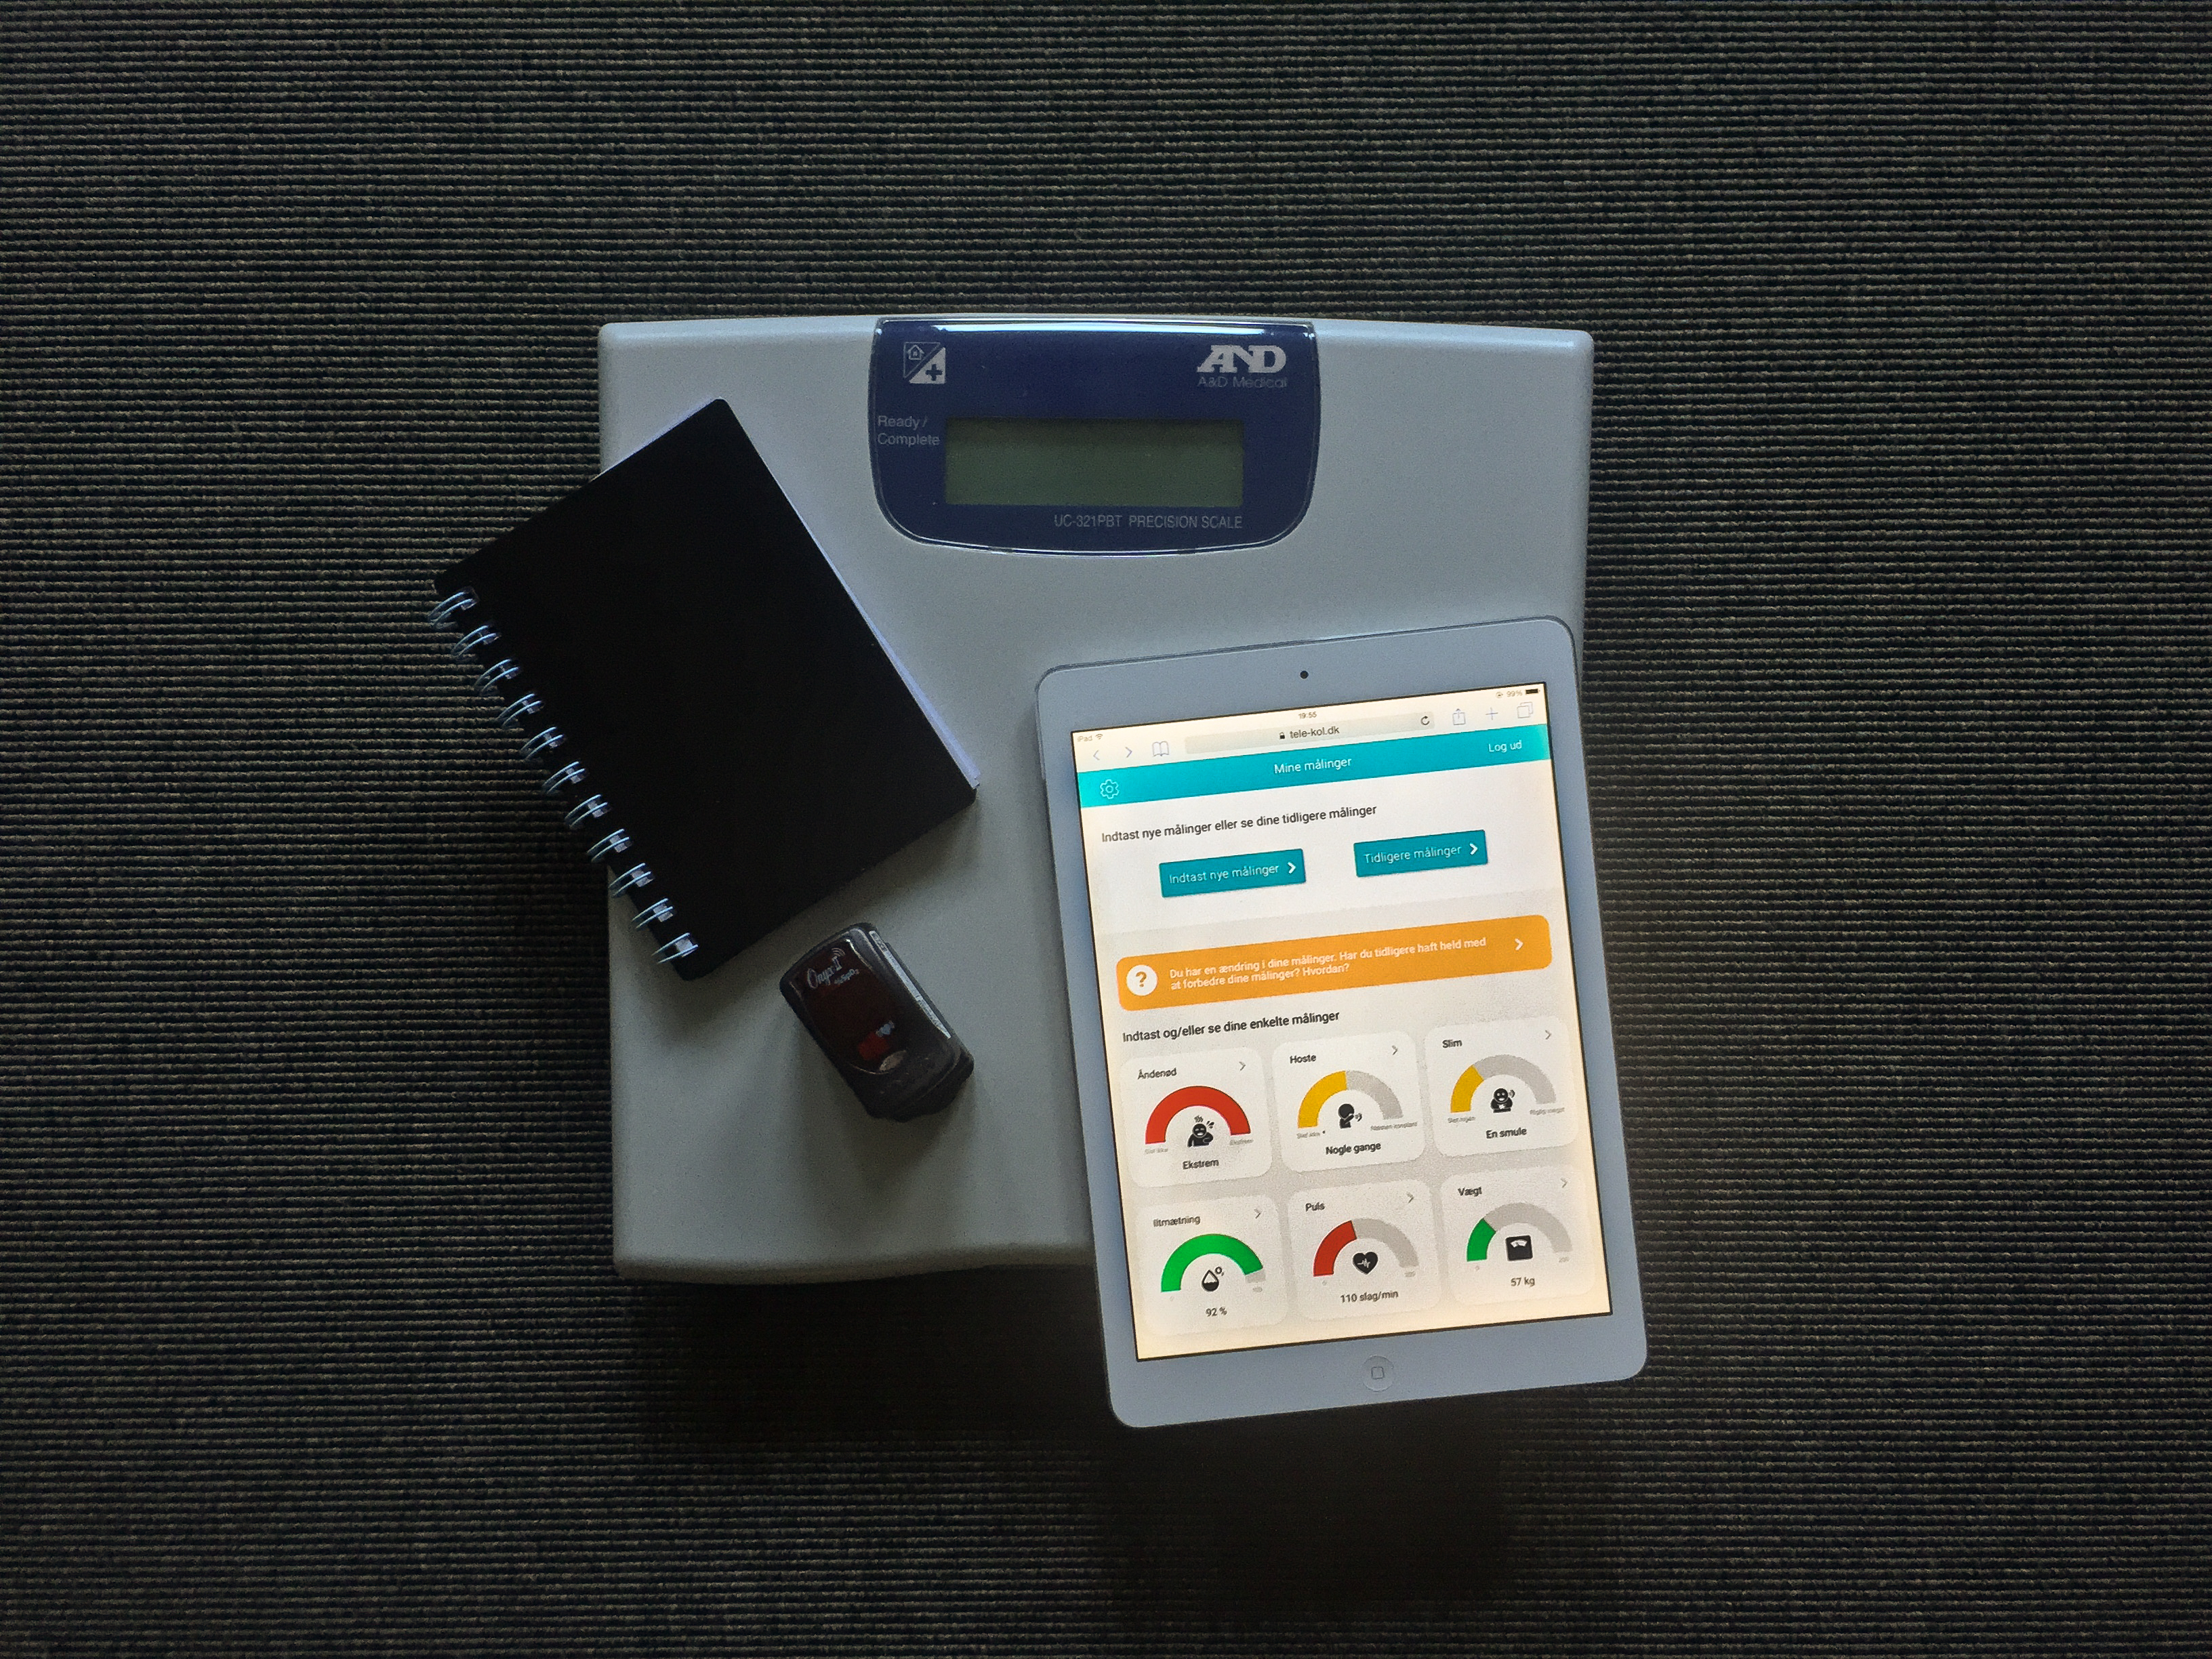
\includegraphics[width=\textwidth]{img/kit}
   %\caption{Flower two.}
 \end{minipage}
  \caption{Patient using TeleKOL (left) and TeleKOL kit (right)}~\label{fig:kit}
\end{figure}


\textit{Debriefs}: Two researchers conducted audio-recorded semi-structured interviews with all patients in their home. Each debrief lasted between 53 minutes and 1 hour and 45 minutes. Before each interview we prepared screenshots of patients' dashboard views showing events of interest (e.g. worsening or improvement in measures between two days) and summaries of log data for each patient used to cue recall in the debrief. While patients filled out demographic questionnaires, one researcher scanned the diaries for events or activities of interest and prepared interview prompts. 

The interview focused on following topics: COPD-related activities for managing disease, context of use and comparison with previous telehealth use. We showed a short video of THC to those patients, who had used it previously, to remind them (since they had not used it for a while) before we engaged in a discussion on comparing their previous telehealth experience with the system they had used. 

Inspired by the grounded theory approach \cite{IDbook}, we transcribed and coded the audio-recordings using an initial code list. We then defined emerging themes through an iterative process of reviewing the codes. We also include findings from the logging and diaries in the following. 

\subsection{Results}
From the analysis, we identified five themes: (1) Barriers for reflection and system use, (2) using measures as health status indicators, (3) feeling empowered in everyday life, (4) questioning and gaining self-knowledge and (5) becoming motivated to self-improve. While some of the themes overlap, there are also noticeable differences related to different levels of reflection. 

\subsubsection{Barriers for Reflection and System Use}
All patients mentioned the agreement with us as the main motivation for taking the system into use, except P3 who mentioned doing it, because she wanted to know her current status (\textit{self-knowledge}) and what she could do about it (\textit{self-improvement}). 

Similar to patient types found in Study 2, passive patients only took the role as data providers when using the system and did not consider it their job to engage in reflective activity of the self-tracked data. We classified three patients (P1, P3 and P4) as active patients and two patients (P2 and P5) as passive patients. 

Passive patients were not motivated to reflect on their own health, \textit{"we can not do anything except measure"} (P2) and \textit{"if the bright minds can not make sure that I get better, then neither can I do anything about it"} (P5). According to P5, reflecting on self-tracked data involved speculating about things that she did not believe she could change, \textit{"I do not worry about things that I can not change"}, but she already engaged in a similar reflective activity in order to change things, e.g. using the pulse oximeter to e.g. adjust her supplemental oxygen level, when she did not feel well.

Frequency and average duration of system use were not indicative of whether patients were classified as active or passive (See Figure \ref{charts}). All patients had used the system approximately 4-5 times, except one active patient (P4) who had used it nine times. Two of the active patients (P1, P4) logged in once during the trial period for the purpose of interacting with visualisations supporting long-term reflection alone. 

\begin{figure*}
 \centering
 \includegraphics[width=2.1\columnwidth]{img/charts}
 \caption{Frequency of use (left) and average duration of use in min/session (right)}~\label{charts}
\end{figure*}

All patients except P1 read and acted on reflective questions (e.g. system asked P4, \textit{"You have several measures that are yellow or red. Have you explored what your measures might have been affected by? (Look into previous measures)"}, wherafter P2 followed the instructions and explored multiple measures and context data). 

Patients used the system on average between 4 minutes and 51 seconds and 12 minutes and 30 seconds per session (M: 9.28), where session refers to logging in, interacting with the system and logging out. The longest session lasted 32 minutes (P4), consisting of entering measures, answering reflective question and interacting with visualisations. The shortest session lasted 3 minutes, consisting of only entering measures (P2 and P4). Both passive patients and one active patient (P3) used approximately 3/4 of the session time on the collection page. 

\subsubsection{Using Measures as Health Status Indicators}
Patients attached importance to their subjective feeling (i.e. how they are feeling) and their engagement in reflective activities on symptom changes depended on whether they felt good or bad. When patients felt good, they did not necessarily see a reason to engage in the reflective activity about symptom change. Revisiting past using the provided time series graph was not of interest to the majority of the patients, which was also reflected in the low usage among patients (except P4). 

Reflecting on the past was negatively charged by P1, \textit{"that's not something I walk around and think about .. Life gets too strenuous if you walk around and think about that [bad days in past]"} (P1). Attaching importance to embrace good days were important to patients, e.g. \textit{"[if] I actually feel good, then I do not worry about how I felt yesterday"} (P3). On the other hand not feeling well in the moment triggered reflection, \textit{"if I do not feel like everything is fine, I might start thinking why (...) it depends on how I am feeling"} (P4). 

Patients already used their pulse oximeter to check their current status, clarify whether oxygen saturation was the cause of not feeling well and then initiated action to improve their condition (e.g. breathing exercises if oxygen saturation measure was too low). The dashboard provided a similar indication of health status using multiple measures, \textit{"it [dashboard] is a measure of one's symptoms (...) altogether it of course becomes how you are feeling"} (P1). 

The self-tracking activity informed and increased the awareness of how patients were feeling, \textit{"I start noticing three times a week, how am I feeling right now?"} (P4). P3 found it helpful to have it visualised on the dashboard what caused her not feeling well, \textit{"you can not even go to the doctor and learn about your status and why (...) that you can do here [dashboard]"} (P3). 

\subsubsection{Questioning and Gaining Self-Knowledge}
In using the system, some patients had gained insights and self-knowledge that they had not previously been aware of. Patients asked themselves questions, increasing their awareness on causes of symptom changes. 

Reflective questions in combination with annotating measure with context variables in the system triggered reflection in P3, who had identified that weather had an impact on her breathing difficulties, \textit{"(..) with dyspnea, I had not thought there could be other [reasons] .. I just had breathlessness, done. (..) suddenly I realized how much I was affected by the heat (...) it happened when I sat with the system and those questions asking 'why?'"}. Annotating with context variables supported evaluating different causal explanation \textit{"I have started thinking about it (...) I think, 'no it's not that [stress]', 'Talk? No I haven't talked today' .. and then I think 'it's the weather'"} (P3).
 
P4 had started reflecting more on the day before and compared it with the presence to assess whether he could improve anything from yesterday, \textit{"I become very conscious about, how did I feel yesterday? Do I also feel like that today?"} (P4).

\subsubsection{Feeling Empowered in Everyday Life}
Using the system had a transformative effect on P3, who had obtained a new perspective on her disease after using the system and an understanding of, what the measures meant. She felt that having COPD in many years had made her passive and lost hope on being able to do something. 

\textit{"My memory has been stuck, so I thought that is just how it is.. You give up a little and get tired of it [COPD] (...) without doing anything about it, because nobody says anything.. but this [the system] does. It makes you aware about the situation (...) My doctor always told me that it is all because of my condition. The system makes me think that he is not right. I might have to make demands, then I might get better."} (P3) 

Some patients (2/5) felt more empowered in planning and overcoming everyday tasks. P3 mentioned not wanting to embarrass herself publicly and felt that she could plan to avoid such situations because of the gained knowledge about how she was affected by the heat, \textit{"now I can make up my mind beforehand [whether to go outside in the heat], because I know how it will end, now when I have been told.."} (P3). Similarly, P4 found that it provided him with a feeling of safety knowing that he was within the recommended levels in terms of his measures, which he could see on the dashboard, \textit{"I'm on the right track then. I do not have to worry about going to folk school or something else"} (P3). 

\textit{Social Responsibility:} Active patients who did not live alone (P3, P4) felt socially responsible towards their relatives. \textit{"I can become unsure about how I am feeling.. (...) I do not want to expose my husband and daughter unnecessary [frightening events] it is about balancing..I learn more about that now, so that I do not expose them [relatives]"} (P3). 

The self-tracking activity made P5 feel egocentric, but he considered it important in order to be able to do what was best for himself and his relatives, \textit{"I have to be self-centred (...) I have to do things right for myself and in time, so that I also treat others right"} (P4). 

\subsubsection{Becoming Motivated to Self-Improve}
Active patients (2/3) started setting goals themselves to improve measures. This involved seeking new knowledge, \textit{"I've tried to acquaint myself with BMI because I wanted to have a goal to follow.. [because] I wondered about the arrows [in the system]"} (P4). 

P3 had not previously been aware of the severity of her weight problems had become aware of the need of improving her condition, \textit{"I have not thought about it before, but when you suddenly get it in writing (...) being confronted with it, I have to do something about it (...) it's for my own good"} (P3). She had started making changes to her eating habits in order to lose weight (eating less, thinking about what she eats, etc.) and mentioned being more aware of engaging in proactive behaviour, \textit{"[less] coughing, that's about getting better at using the PEP device.. Not just saying, ‘oh, you are running into a pneumonia, now you have to use it', it's about using it [PEP device] several times a day"}. 

Some patients used the color indicators and arrows in combination as indicators of status and used them as goals,  \textit{"I want all of them to be green and that things are making progress"} (P3) and \textit{(...) when the arrows are pointing down I assume it is not so good, that's the wrong way"} (P4). Seeing the progress in the system and that it paid off to change her behaviours, motivated P3 to ease off medication intake, which she had tried several times in the past without success. \textit{"They had difficulties easing me off because I have had high doses for so many years (..) but this time I thought (...) now you have to stop (...) I did .. I needed some days and then it was over"} (P3). 

\textit{Actionable Advice}: Both P1 and P3 requested actionable advice on what they could do to improve their conditions. P3 needed advice on how to progress towards her goal of losing weight taking into account her other health-related conditions \textit{"to get help when you also have diabetes, that would be nice"}. P1 mentioned needing actionable advice on improving measures, \textit{"when you sit alone, have breathing difficulties, you cough and you have phlegm, you think, what can I do? It is the alpha and omega"}. 

\section{Discussion} 
We investigated how concrete design decisions regarding entry and interaction with data affected reflection in telehealth among COPD patients. Our findings indicate that active patients benefited by becoming more informed and aware about their health status using the features in the system, leading to increased empowerment in their everyday life and motivation to self-improve by setting goals. In contrast, passive patients were not interested in reflecting on their self-tracked data, but the lacking motivation to reflect on data was not a barrier for their engagement with the system (e.g. only little difference in frequency and average duration of use between active and passive patients). 

Previous literature shows conflicting results in terms of effectiveness of telehealth interventions for COPD patients on utilization of healthcare services and health-related quality of life  \cite{pedone}. We found that patients were highly motivated to log and submit data, because it provided them with sense of security to be monitored by a healthcare provider. However, we also observed an implication in current telehealth design, where some patients lacked knowledge or awareness on submitting reliable and valid measures, potentially hindering healthcare professionals in the early detection and initiation of treatment (the purpose of telehealth). 

Our findings suggest that some patients did not want to be confronted with a past that cannot be changed, whereas visualising discrepancies that can be changed, encouraged some active patients to set goals in order to self-improve. Whether patients in fact become more self-managing requires a long-term study on behaviour change. While we provided patients with visualizations of past (history data) with the purpose of supporting reflection on change over time \cite{Rivera, Cuttone} and patients mentioned benefits in seeing improvements in their measures, we found low usage of such visualizations in the real context, unless patients were curiosity-driven. Previous studies found that self-tracked data reminded people with a chronic health condition of negative aspects of their condition \cite{Li2010, Ancker2015}, which could explain our findings in relation to passive patients. Personal Informatics literature often mention simple visualisation of history as the method for supporting reflection \cite{Li2011, MacLeod2014, Rivera}, but considering the negative effects it can have on people with a deteriorating chronic condition (already suffering from anxiety and depression), we propose that future research investigates design to support seeing the positive and its effects. 

We found that designing for discrepancies (color indicators and arrows) and questioning (reflective questions in the system) triggered awareness and encouraged exploring different causal explanations (R2, higher level of reflection \cite{Fleck}) among some active patients. Whether this also makes it possible for patients to detect onsets of exacerbations earlier is yet to be investigated. It is further unclear whether outcomes will be the same, if a healthcare provider monitors the data as in real telehealth. 

Supporting previous literature on conditions for reflection \cite{Atkins, Rogers}, our findings show that passive patients were not open-minded or motivated toward engaging in reflection on their data, making it a barrier for them to benefit from the designed features. Additionally, both passive patients in the study had limited experience in interacting and using a tablet, which might have been another barrier. Fleck \& Fitzpatrick suggest that people need a reason or encouragement in order to engage in reflective activity \cite{Fleck}. In order to motivate passive patients to take a more active role in their own health, it might be necessary to consider other interventional methods or provide further support in the system to intrinsically motivate passive patients. 

Some patients were highly motivated to engage in reflection and even started setting goals to self-improve, using features in the system as goals. However, similar to Epstein et al., our findings suggest that lacking knowledge or support (e.g on how to improve measures) can be a barrier for self-improvement (action) \cite{Epstein2015}. While only three of the five participants were active and engaged in the reflective activity, the study might have been subject to self-selection bias. Particularly, the patient who gained most out of the self-tracking activity, had no previous experience with telehealth and thus no experience with the benefits of self-tracking (e.g. gaining self-knowledge). Patients might have been more reflective, because we primed them to reflect by telling them the purpose of the study and asked questions during the debriefs that prompted reflection. As mentioned by Isaac et al., reflection can be triggered when trying to externalize thoughts or feelings, e.g. in diaries. In our study, the use of diaries as a data collection method might also have fostered additional reflection \cite{Isaac}. 
 
\section{Conclusion}
Our study explores self-tracking needs in telehealth and how concrete design choices affects reflection among COPD patients. We investigated user needs and concerns critical for the effectiveness of telehealth interventions using a synthesis of literature on Personal Informatics and analysis of interviews with COPD patients using a state of the art telehealth solution. While patients generally felt taken care of, our findings show that some patients were not providing reliable and valid data, either due to lack of knowledge or awareness. Neither did the system support reflection on the self-tracked data or any follow-up action. 

Interviews, workbooks and feedback sessions informed the redesign of the telehealth system. We designed and developed a prototype to support self-reflection among the patients and evaluated it in a two week field trial. Our findings show that using simple color indicators and arrows for visualising discrepancies and asking reflective questions in the system can be a first step towards increasing active patients' self-awareness on their health status. Future researchers should investigate, how to support and motivate patients (both active and passive) e.g. through actionable advice to meet their self-tracking needs. 

\section{Acknowledgements}
We would like to extend our gratitude to the staff at Silkeborg Regional Hospital and Center for Telemedicin in Aarhus for their help and collaboration. Thanks to all participants whose consent and involvement enabled the conduct of this research. We  would also like to express our appreciation to our supervisor Hendrik Knoche for his advice and assistance.

%\input{design}
%\section{Experiment}

\subsubsection{Hypothesis}
We hypothesized that 

\textbf{H0:} 

\hspace{10 mm} \textit{H0: $\mu$EnjoyabilityRiddle $\leq$ $\mu$EnjoyabilityMap}

\textbf{H1:} Riddle solving as navigational method is more enjoyable than maps.

\hspace{10 mm} \textit{H1: $\mu$EnjoyabilityRiddle $>$ $\mu$EnjoyabilityMap}

\subsubsection{Participants}


\subsubsection{Materials and Procedure}

 
\section{Results}


%\section{Discussion}

critical: ensure validity in a questionnaire, for instance originally in English translated to Danish. No content validity index was computed? 




Effect of TH less effective for participants with mild or moderate COPD
%\input{conclusion}
%\section{Acknowledgements}
We would like to extend our gratitude to the staff at Silkeborg Regional Hospital and Center for Telemedicin in Aarhus for their help and collaboration. Thanks to all participants whose consent and involvement enabled the conduct of this research. We  would also like to express our appreciation to our supervisor Hendrik Knoche for his advice and assistance.

%\cite{AugmentingAudioMessages} \cite{Carrigy:2010:DEP:1868914.1868929} \cite{DesigningMobileARI} \cite{GamingTourism} \cite{HideAndSeek} \cite{InterdisciplinaryCriticism} \cite{JCAL:JCAL316} \cite{Klemmer:2002:WSC:503376.503378} \cite{LostLab} \cite{Mather:2000:MUT} \cite{Savannah} \cite{Schwartz:1995:GBF} \cite{StoryTrek} \cite{TheoreticalAndMethod} 

% Balancing columns in a ref list is a bit of a pain because you
% either use a hack like flushend or balance, or manually insert
% a column break.  http://www.tex.ac.uk/cgi-bin/texfaq2html?label=balance
% multicols doesn't work because we're already in two-column mode,
% and flushend isn't awesome, so I choose balance.  See this
% for more info: http://cs.brown.edu/system/software/latex/doc/balance.pdf
%
% Note that in a perfect world balance wants to be in the first
% column of the last page.
%
% If balance doesn't work for you, you can remove that and
% hard-code a column break into the bbl file right before you
% submit:
%
% http://stackoverflow.com/questions/2149854/how-to-manually-equalize-columns-
% in-an-ieee-paper-if-using-bibtex
%
% Or, just remove \balance and give up on balancing the last page.
%
\balance

\bibliographystyle{acm-sigchi}
\bibliography{references}
\end{document}
